\section{Introduction and Motivation}



% Intro
% * Hva skjer
% * Hvorfor er dette et problem
% * Kan vi gjøre noe med det?
% * Hva gjør vi for å komme nærmere en løsning
% * Hva har vi fått til
% * Noe ekstra dette kan brukes til




% Hva skjer
As we are standing on the doorstep of the ages of Dark Silicon, increased energy
efficiency is a key factor to allow more performance.
\autoref{fig:cpuperformace} tells us how single-threaded performance almost
halted as we hit the power wall. Because of the end of Dennard scaling, further
shrinking of the transistor did not shrink the power dissipated by each one of
them. This leads to a rapid increase in power denisty, and if the industry
continues cramming more logic to single threaded performace, wattage per area
would be too high for common cooling techniques.

With the mentioned problems in mind, more energy efficient ways of doing common
tasks will be a key to allow further expansion of the hardware.  Since the
entire chip cannot be powered at once, it is more and more common to let parts
of the chip be specialized for a specific task. This is a major research area
for the SHMAC-project, which aims to create an energy efficient composition of
specialized as well as general purpose processing tiles. This thesis will
look more towards how the dynamic energy consumption can be further decreased
by creating a tool which can evaluate different processor features before they
are realized.

From the research performed in \cite{rundehvatum2013exploring} we have found
that different instructions consume a slightly different amount of energy.
\autoref{fig:consumptioncond} shows some results showing how conditional
execution affects energy consumption, while \autoref{fig:consumptionmulti}
shows that different execution times affects the total energy spent. Base
refers to the cheapest instruction found in the instruction set, \texttt{setned}.
\texttt{setend} is used here just to set the same endianess as already set,
and thus it flushes the processor without doing anything else.


\begin{figure}{tbh}
\begin{subfigure}[b]{0.48\textwidth}
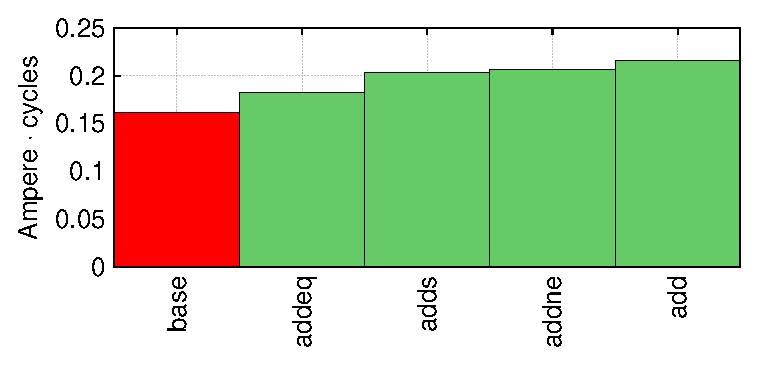
\includegraphics[width=\textwidth]{graph_01_base_cond-0c6.eps}
\caption{Conditional execution (eq is false).}
\label{fig:consumptioncond}
\end{subfigure}
\begin{subfigure}[b]{0.52\textwidth}
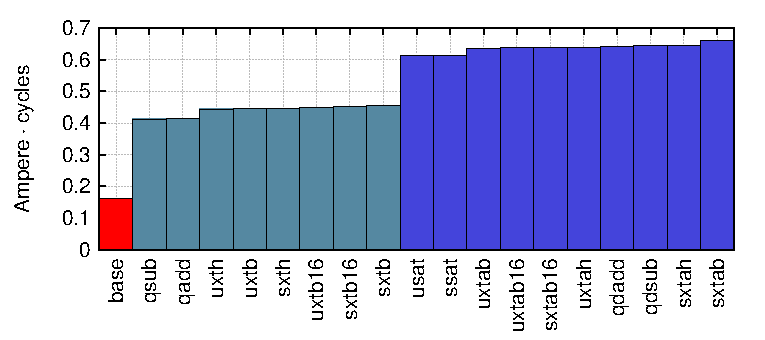
\includegraphics[width=\textwidth]{graph_023_base_quad_saturate_extend-0c6.eps}
\caption{Non-multiply multi-cycle instructions.}
\label{fig:consumptionmulti}
\end{subfigure}
\caption{Figures from \cite{rundehvatum2013exploring} showing the results of measuring the
current drain through the CPU core while running isolated instructions in a loop.}
\label{fig:consumption}
\end{figure}

